\chapter{Desenvolvimento}
\label{c.desenvolvimento}

\section{Modelo Teórico e estrutura modular}
\label{s.modeloteorico}

Seguindo a abordagem descrita por \citeauthoronline{canoetal05} (\citeyear{canoetal05}) foi desenvolvido um módulo para cada fase dos processos de extração do \emph{audio fingerprint}:

\begin{alineas}

\item Pré-processamento
\item Enquadramento
\item Transformada
\item Extração de características
\item Pós-processamento
\item Modelagem do fingerprint

\end{alineas}

Cada etapa é um módulo independente que passa a informação tratada através de stream de audio ou arquivo para a próxima etapa até a obtenção do \emph{audio fingerprint} final. Uma etapa anterior foi adicionada para extrair o audio de uma fonte web e enviar para o sistema de geração de \emph{audio fingerprint}.


\begin{figure}[h]
\caption{\small Ambiente de desenvolvimento da aplicação do modelo teórico.}
\centering
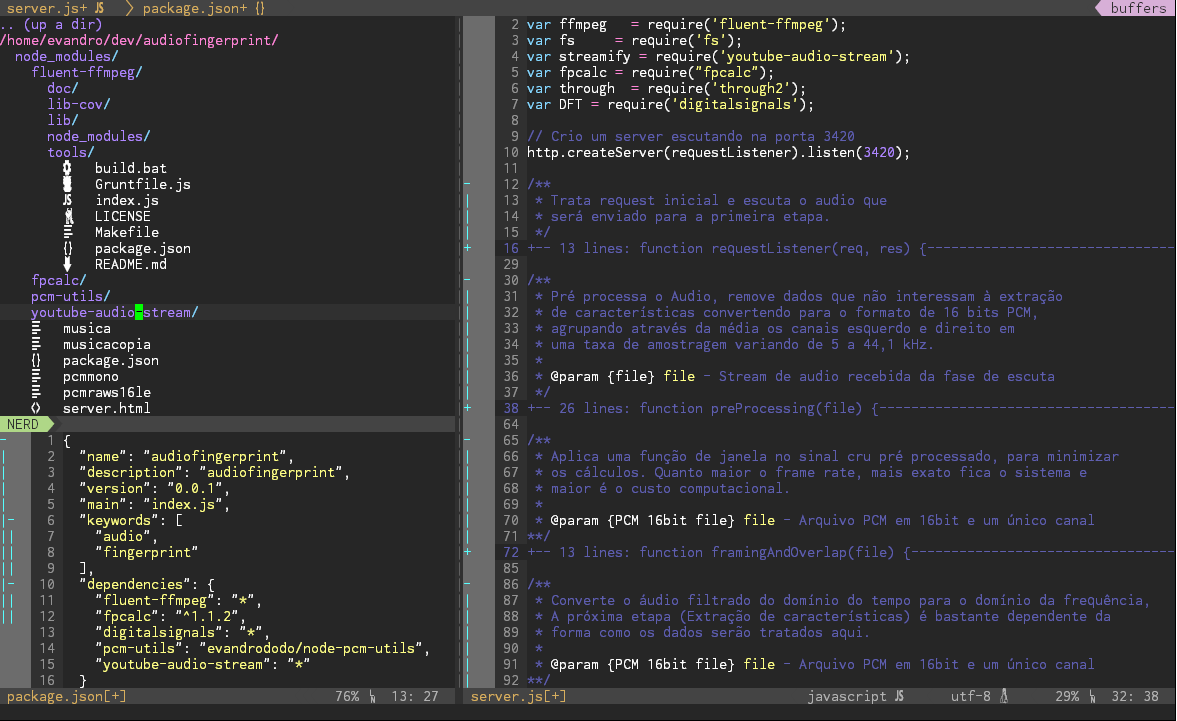
\includegraphics[scale=0.50]{figs/ambientegeral.png}
\label{f.diagrama}
\legend{\small Fonte: Elaborada pelo autor.}
\end{figure}

\subsection{Pré-processamento}
\label{ss.preprocessamento}

Pré processa o Audio, converte para o formato de 16 bits PCM, e agrupa através da média os canais esquerdo e direito em uma taxa de amostragem variando de 5 a 44,1 kHz.
	
\begin{verbatim}
function preProcessing(file) {
    // Cria um stream de leitura com base no arquivo que esá
    //  recebendo a musica em PCM
    var preProcStream = fs.createReadStream(file),
        pcmMono = fs.createWriteStream('pcmmono'),
        musica = '';

    preProcStream.on('data', function(chunk) {
        console.log(chunk.length);
        musica += chunk;
    });

    preProcStream.on('end', function(chunk) {
        console.log('Iniciando conversão para PCM...');
        ffmpeg(__dirname + '/musicacopia')
        .format('pulse')
        .audioChannels(1)
        .output(__dirname + '/pcmmono')
        .on('end', function() {
            console.log('Música convertida para PCM 16bits Mono');
            framingAndOverlap(__dirname + '/pcmmono');
        })
        .run();
    });
} 
\end{verbatim}	

\subsection{Enquadramento}
\label{ss.enquadramento}

Aplica uma função de janela no sinal cru pré processado, para minimizar os cálculos. Quanto maior o frame rate, mais exato fica o sistema e maior é o custo computacional.

\begin{verbatim}
function framingAndOverlap(file) {
  var preProcStream = fs.createReadStream(file),
      frameSize = 4096, 
      overlap = 75, //porcentagem
      fao = new framingAndOverlap();
      
      fao.size(frameSize).overlap(overlap).run(preProcStream);
      transformada(file);
}
\end{verbatim}


\subsection{Transformada}
\label{ss.transformada}

Converte o Audio filtrado do domí­nio do tempo para o domí­nio da frequência,  a próxima etapa (Extração de caracterí­sticas) é bastante dependente da forma como os dados serão tratados aqui.
	
\begin{verbatim}
function transformada(file) {
  var procSinal = fs.createReadStream(file),
      dftStream = fs.createWriteStream(__dirname + '/dft'),
      dft = new DFT(1024, 44100);
  dft.forward(procSinal);
  var spectrum = dft.spectrum;
  spectrum.pipe(dftStream);
  extracao(dtStream);
}
\end{verbatim}


\subsection{Extração de Características}
\label{ss.extracaocaracteristicas}

A extração de características deve ser ajustada para a finalidade desejada do \emph{audio fingerprint}. No caso de reconhecimento de voz ou instrumentos, os dados mais relevantes são os referentes às frequências com maior indíce de repetição (harmônicas presentes). No caso de reconhecimento de músicas os dados relevantes são a repetições de refrões, melodia e \emph{chroma} musical.

\begin{verbatim}
function extracao(stream) {
  var sinalfreq = fs.createReadStream(stream);

    // Análise simplificada do sinal sonoro: contando as frequencias
    // que mais se repetem (harmonicas de instrumento)
    sinalfreq.on('end', function(chunk) {
        console.log('Contando frequências do sinal e agrupando');
        var coordFN = sinalfreq;
        // Envia a contagem para o pós processamento como um vetor
        // de distância em N dimensões, sendo N o número de 
        // frequências disponíveis
        posprocess(coordFN);
    });
}
\end{verbatim}


\subsection{Pós-processamento}
\label{ss.posprocessamento}

Para gerar um fingerprint o dado com as características relevantes deve ser normalizado e pode ser simplificado atraves de derivadas de primeira e segunda ordem.

\begin{verbatim}
function posprocess(coords) {
  var maxFreq = -11000,
      minFreq = 11000;
   for(int i=0;i<coords.length;i++) {
       if(coords[i]<minFreq) {
           minFreq = coords[i];
       }
       if(coords[i]>maxFreq) {
           maxFreq = coords[i];
       }
    }
    var amplitude = maxFreq - minFreq,
       intervalo = amplitude/36; //26 letras e 10 numeros
    // Normalizando o sinal para 36 representações
   for(int i=0;i<coords.length;i++) {
       coords[i] = Math.round(coords[i]/intervalo);
    }
    modeling(coords);
}
\end{verbatim}

\subsection{Modelagem do Fingerprint}
\label{ss.modelagemfingerprint}

A modelagem do fingerprint usualmente recebe uma sequência de vetores de características. Através desse vetor é gerado um hash de identificação.

\begin{verbatim}
function modeling(coords) {
    var simbolos = ["a", "b", "c", "d", "e", "f", "g", "h", "i", "j", "k", "l",
     "m", "n", "o",     "p", "q", "r", "s", "t", "u", "v", "w", "x", "y", "z",
      "0", "1", "2", "3", "4", "5", "6", "7", "8", "9"];
        hash = ""';
   for(int i=0;i<coords.length;i++) {
     hash = hash + simbolos[coords[i]];
    }
    console.log('Hash de identificação:');
    console.log(hash);
}
\end{verbatim}

\section{Geração de hash com modelo de contagem de frequências}
\label{s.teste}

Com base no algoritmo modular desenvolvido foi gerado um hash para teste de eficiência de processamento, esses módulos podem ser modificados para atender vários modelos de \emph{audio fingerprint}. Como exemplo as transformadas DFT podem ser substítuidas por transformadas Wavelet e o vetor pode ser resumido à derivativa de primeira ordem, dependendo da finalidade da aplicação.

\begin{figure}[h]
\caption{\small Teste de geração de hash simples.}
\centering
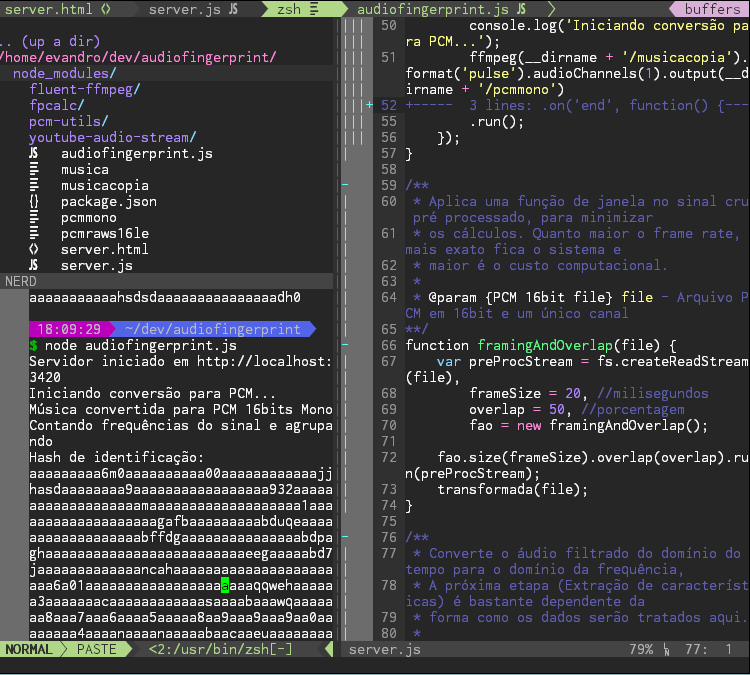
\includegraphics[scale=0.75]{figs/execucao.png}
\label{f.execucao}
\legend{\small Fonte: Elaborada pelo autor.}
\end{figure}

\section{Base de dados e reconhecimento de músicas}
\label{s.basedados}

Para catálogo de músicas e artistas existentes foi utilizado o banco de dados da MusicBrainz, que disponibiliza um script de backup e criação de um banco \emph{PostgreSQL}. Os dados deste banco estão em domínio público e a MusicBrainz disponibiliza também um servidor que sincroniza os dados à cada uma hora.

\begin{figure}[h]
\caption{\small Organização do banco de dados do MusicBrainz.}
\centering
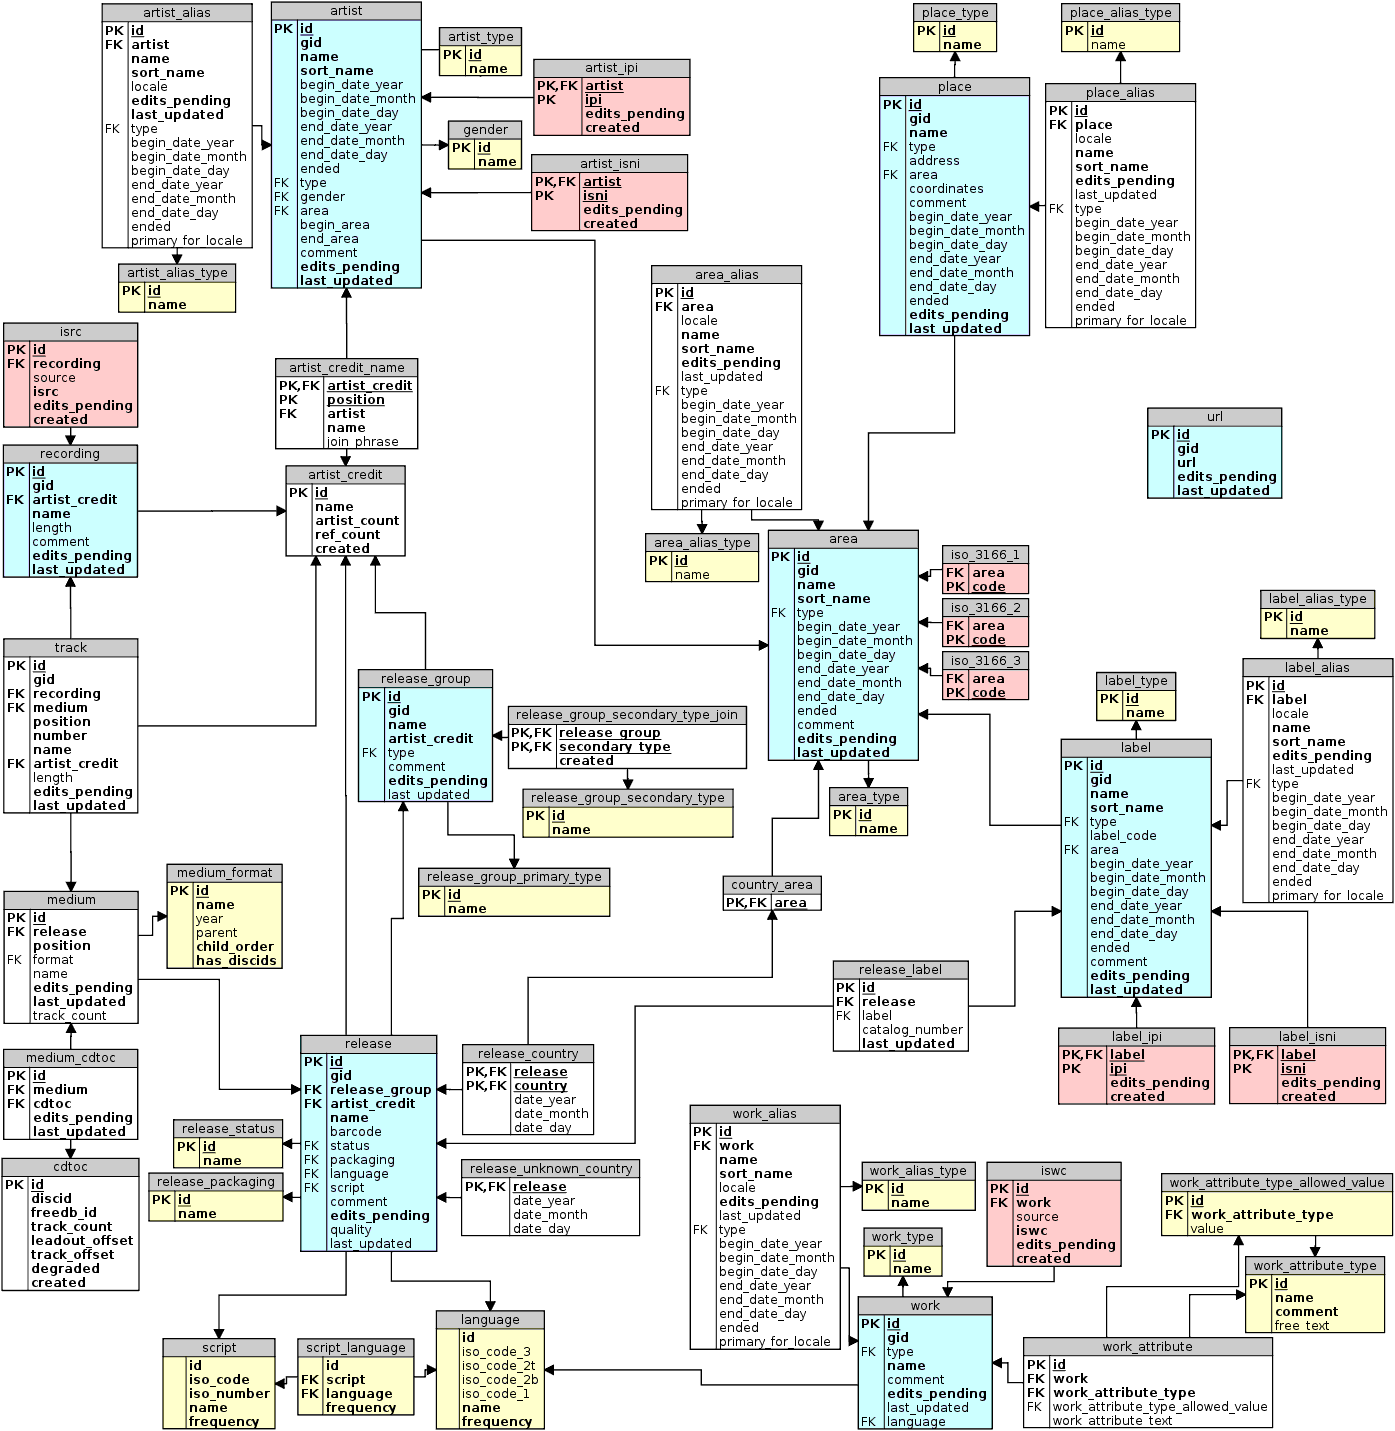
\includegraphics[scale=0.40]{figs/musicbrainzschema.png}
\label{f.musicbrainz}
\legend{\small Fonte: \cite{musicbrainzcite}.}
\end{figure}
 
 Inicialmente foi utilizado um banco de dados local para consulta e treinamento do algoritmo de hash, na fase final de reconhecimento de música a consulta remota em outra máquina se mostrou mais eficiente.
 
\section{Geração de hash \emph{Chroma-based}}
\label{s.hashchroma}

Para a geração de hash para consulta de músicas foi utilizado o algoritmo de \emph{Chromaprint}, descrito na seção \ref{s.chromaprint}. O algoritmo gera um hash representado em caracteres alfanuméricos que pode ser utilizado para consulta nos bancos de dados disponíveis. 

\begin{figure}[h]
\caption{\small Geração de hash com algoritmo de \emph{Chromaprint}.}
\centering
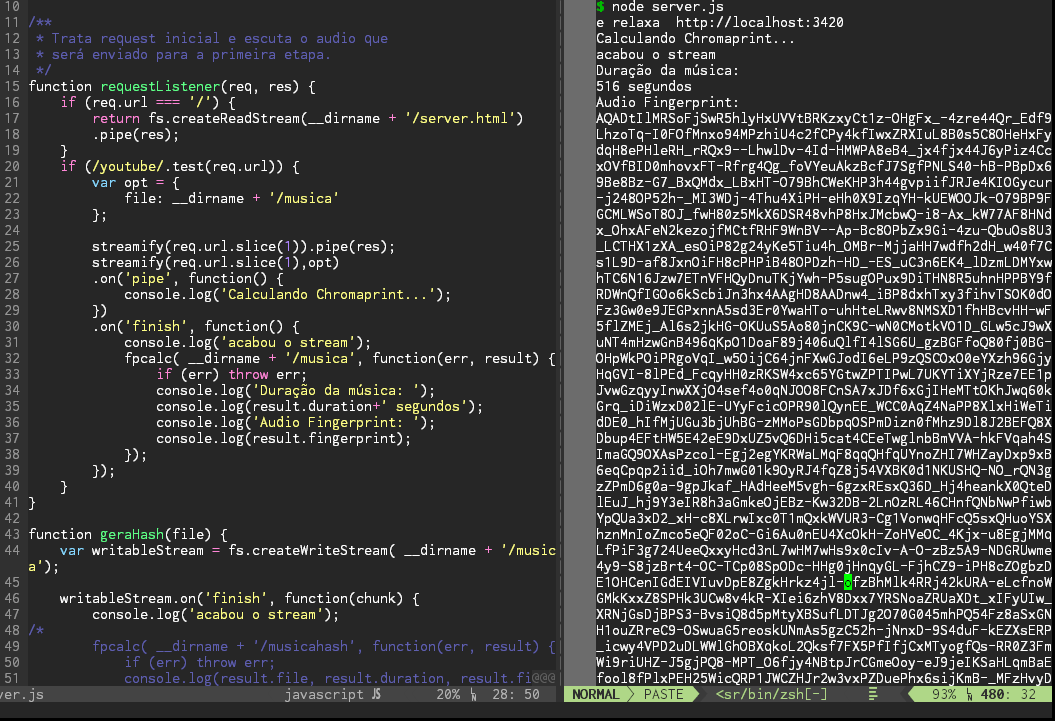
\includegraphics[scale=0.60]{figs/hashchromaprint.png}
\label{f.musicbrainz}
\legend{\small Fonte: Elaborada pelo autor.}
\end{figure}
 

\section{Busca, acesso e teste de acertos}
\label{s.buscanobd}

Com o hash representando o \emph{audio fingerprint} o último passo necessário para o reconhecimento é a consulta no banco de dados. Para a busca, acesso e teste de acertos foi utilizada a base disponibilizada \cite{musicbrainzcite} e o  \emph{web service} da AcoustID, com acesso e comparação através do hash enviado:

\begin{figure}[h]
\caption{\small Busca no banco de dados.}
\centering
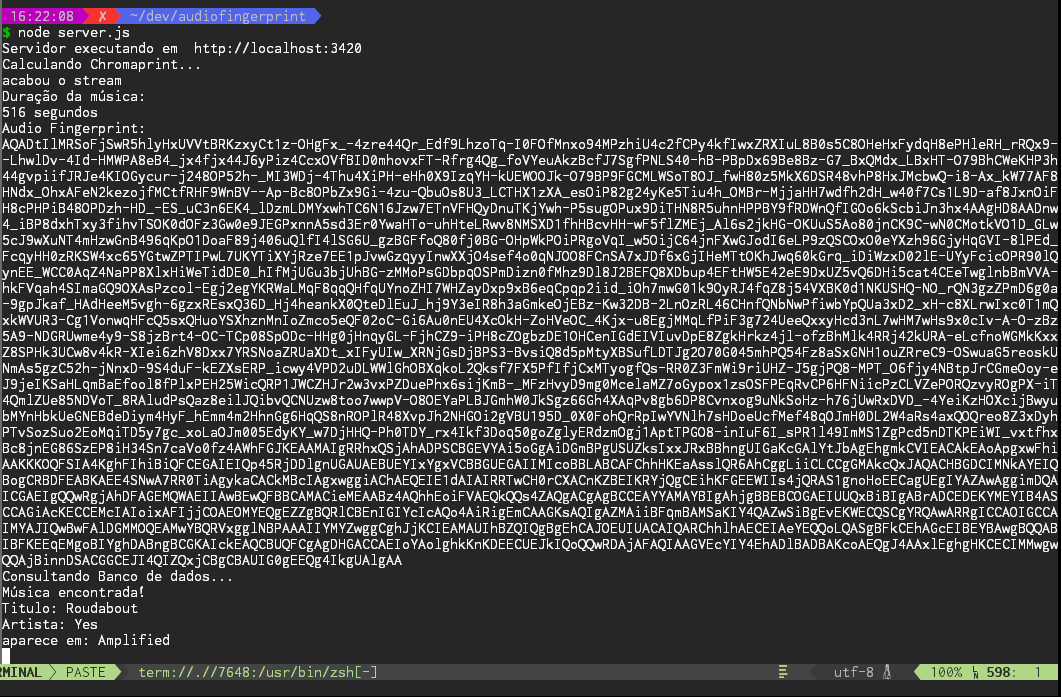
\includegraphics[scale=0.60]{figs/yes.png}
\label{f.musicbrainz}
\legend{\small Fonte: Elaborada pelo autor.}
\end{figure}
 